\newpage % Rozdziały zaczynamy od nowej strony.
\cleardoublepage % Zaczynamy od nieparzystej strony
\pagestyle{headings}

\section{Wybór sprzętu}

\subsection{Xilinx Zynq-7000}

Przy wyborze płytki wzięto pod uwagę posiadane interfejsy oraz cenę sprzętu i dostępność dokumentacji. Podjęto decyzję o zastosowaniu układu FPGA firmy \emph{Xilinx} z racji na duże wsparcie techniczne. W celu optymalizacji kosztów systemu wybrano podstawowe dwa układy z rodziny \emph{Zynq-7000 SoC Family} (Rys. \ref{zynq7000}) XC7Z010 oraz XC7Z020. Aby mieć pewność, że parametry układu będą wystarczające, wybrano układ XC7Z020. 

\begin{figure}[h]
  \centering
  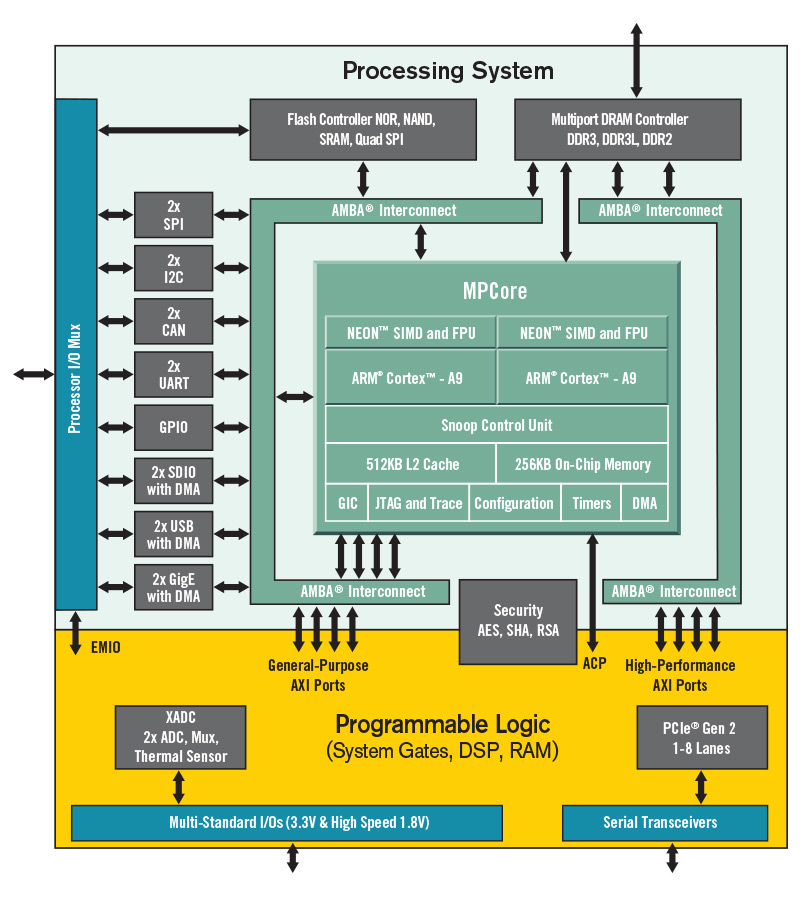
\includegraphics[width=\textwidth]{img/zynq7000.png}
  \caption{Architektura serii ZYNQ-7000 SoC}
  \label{zynq7000}
\end{figure}

Zgodnie z porównaniem zawartym w Tabeli \ref{tab:ceny}, płytka Z-turn Board MYS-7Z020-C-S ma cenę sporo mniejszą od innych płytek z układem XC7Z020. Na stronie producenta można znaleźć pełną dokumentację dotyczącą płytki Z-turn. Wadą płytki jest małe zaangażowanie społeczności w projekty z jej wykorzystaniem, jednak tak konkurencyjna cena ułatwiła podjęcie wyboru.

\begin{table}[h] \centering
  \caption{Porównanie cen płytek z układami Zynq firmy Xilinx}
  \centering
  \begin{tabular} {c|c|c} \hline \label{tab:ceny}
      Nazwa płytki & Układ SoC & Cena \\ \hline
      Z-turn Board MYS-7Z010-C-S & XC7Z010-1CLG400C & 99\$\tablefootnote{http://www.myirtech.com/list.asp?id=502} \\ 
      Z-turn Board MYS-7Z020-C-S & XC7Z020-1CLG400C  & 119\$\footnotemark[1] \\
      Zybo Z7-10 Development Board & XC7Z010-1CLG400C & 199\$\tablefootnote{https://store.digilentinc.com/zybo-z7-zynq-7000-arm-fpga-soc-development-board/} \\
      Zybo Z7-20 Development Board & XC7Z020-1CLG400C & 299\$\footnotemark[2] \\
      ZedBoard Zynq-7000 & XC7Z020-CLG484-1 & 449\$\tablefootnote{https://store.digilentinc.com/zedboard-zynq-7000-arm-fpga-soc-development-board/} \\
  \end{tabular}
\end{table}


\subsection{Z-turn Board}

Z-turn Board (Rys. \ref{zturn_board} jest komputerem jednopłytkowym 
(ang. SBC – \emph{Single Board Computer}), opartym o układ SoC Xilinx 
Zynq-7020 (XC7Z020-1CLG400C), zawierającym dwurdzeniowy procesor ARM Cortex-A9 (866MHz)
i układ FPGA Artix 7. Parametry układu FPGA przedstawiono w Tabeli \ref{tab:artix}.

\begin{table}[h] \centering
  \caption{Specyfikacja techniczna układu Artix-7 }
  \centering
  \begin{tabular} {c|c|c|c|c} \hline \label{tab:artix}
      Logic Cells & LUT & Flip-Flop & BRAM (ilość bloków po 36Kb) & DSP \\ \hline
       85K & 53200 & 106400  & 4.9Mb (140) & 220 \\ 
  \end{tabular}
\end{table}

Producentem płytki jest firma MYIR Tech Limited (ang. \emph{Make Your Ideas Real} ), dostarczająca sprzęt bazujący na 
procesorach ARM oraz oprogramowanie do swoich produktów\cite{myir}. Biorąc pod uwagę parametry, płytka charakteryzuje się 
wysokim stosunkiem ceny do jakości, podstawowa wersja kosztuje 99\$. Dla porównania płytka Zybo Z7-20 kosztuje 199\$. Zaletą 
płytek firmy \emph{Digilent} (ZedBoard i Zybo) jest duże wsparcie producenta i spora ilość materiałów szkoleniowych.

\begin{figure}[h]
  \centering
  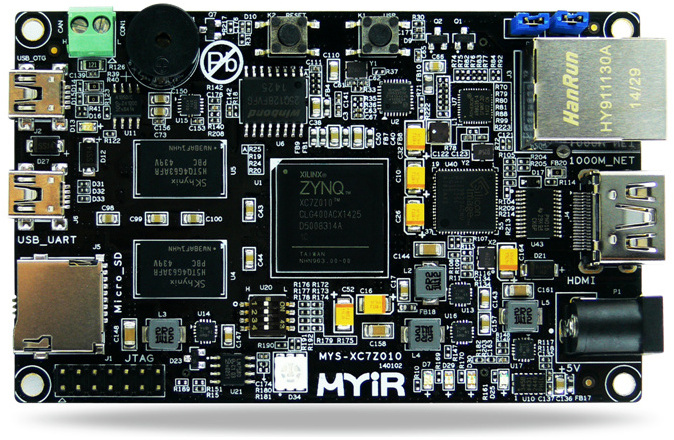
\includegraphics[width=0.8\textwidth]{img/zturn_board.jpg}
  \caption{Płytka Z-turn-Board 7020}
  \label{zturn_board}
\end{figure}


\subsubsection{Interfejsy komunikacyjne}

Płytka Z-turn posiada interfejsy UART oraz Ethernet, które zostały wykorzystane do komunikacji komputera PC z systemem przy 
użyciu portu szeregowego  
i protokołu SSH (ang. \emph{Secure Shell}). Istnieje również możliwość podłączenia wyświetlacza bezpośrednio do płytki przy 
użyciu portu HDMI oraz innych peryferiów przy użyciu portu USB. Dodatkowo producent oferuje płytkę rozszerzeniową Z-turn 
IO-Cape (Rys. \ref{iocape}), która zawiera porty do podłączenia kamery przez protokół DVP (ang. \emph{Digital Video Port}) 
oraz wyświetlacza LCD. 

\begin{figure}[h]
  \centering
  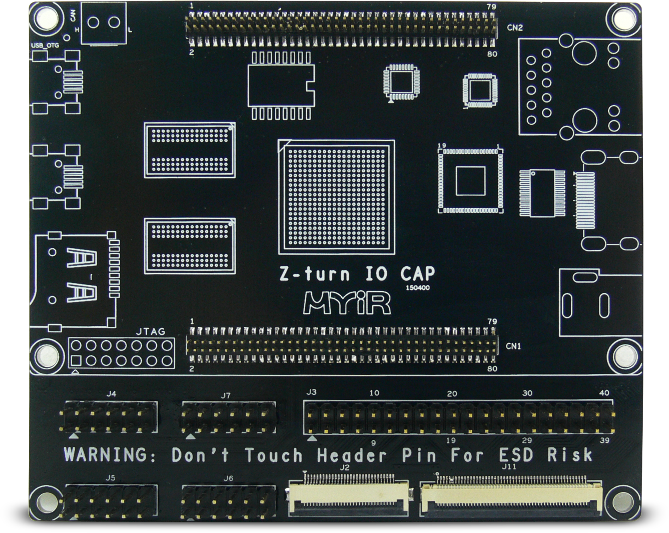
\includegraphics[width=0.8\textwidth]{img/iocape.png}
  \caption{Płytka rozszerzeniowa Z-turn IO Cape}
  \label{iocape}
\end{figure}

\subsection{Kamera}

Aby przetestować działanie systemu w czasie rzeczywistym, wykorzystano zewnętrzny 
moduł kamery. Przy wyborze sprzętu istotna była ceną modułu, interfejs komunikacji
oraz kompatybilność z SBC Z-turn Board. W przypadku wykorzystania kamery w czasie 
rzeczywistym bardzo ważne jest niskie opóźnienie w wysyłaniu kolejnych ramek obrazu i duża szybkość transferu obrazu. 

Producent płytki Z-turn Board oferuje kilka modułów kamer. Wśród nich znajdują się dwa moduły, które zostały przetestowane: 
MY-CAM002U USB Digital Camera Module (Rys.\ref{cam-usb}) oraz MY-CAM011B BUS Camera Module. (Rys. \ref{cam-dvp}). W Tabeli 
\ref{tab:kamery} przedstawiono porównanie testowanych modułów kamer. 

\begin{table}[h] \centering
  \caption{Porównanie testowanych modułów kamer}
  \centering
  \begin{tabular} {c|c|c} \hline \label{tab:kamery}
      & MY-CAM011B &  MY-CAM002U \\ \hline
      Maksymalna rozdzielczość & 1600x1200 pikseli & 1280x800 pikseli \\ \hline
      Pobór mocy w stanie aktywnym & 224 mW & 110 mW\\ \hline
      Format wyjścia & 8/10-bit RAW RGB & 10-bit RAW RGB \\
      & YUV422/YCbCr422 & \\
      & RGB565/555 & \\
      & GRB422 & \\ \hline
      Maksymalny transfer obrazu & 15 fps (1600x1200)  & 30 fps (1280x800) \\
      & 30 fps (800x600)  & 60 fps (640x480) \\
      & 30 fps (1280x720) & 30 fps (1280x720) \\
      & 24 fps (1366x768) & \\ \hline
      Cena modułu & 25\$\tablefootnote{http://www.myirtech.com/list.asp?id=534} & 19\$\tablefootnote{http://www.myirtech.com/
      list.asp?id=462} \\
    \end{tabular}
  \end{table}
  
  \begin{figure}[!h]
      \centering
      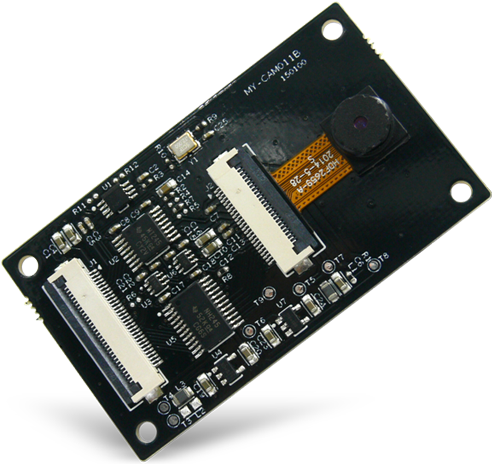
\includegraphics[width=0.7\textwidth]{img/my-cam011b.png}
      \caption{Moduł kamery MY-CAM011B BUS Camera Module}
      \label{cam-dvp}
    \end{figure}

\subsubsection{Moduł MY-CAM011B}

Kamera MY-CAM011B zapewnia większą rozdzielczość maksymalną i posiada interfejs równoległy DVP. Skutkuje to mniejszymi 
opóźnieniami w wysyłaniu kolejnych ramek obrazu niż w przypadku kamery MY-CAM002U, podłączanej przez USB. 

Pomimo znajdującego się na płytce IO-Cape portu interfejsu DVP, moduł kamery MY-CAM011B niestety okazał się niekompatybilny z 
płytką Z-turn Board. Na schemacie płytki rozszerzeniowej IO-Cape widać (Rys. \ref{cam-schematic}), że sygnał zegara 
(CAM\_XCLK) nie jest dołączony do żadnego portu płytki Z-Turn Board. Piny CAM\_PWRDN i CAM\_RST również nie są dołączone do 
złącza J2 od strony płytki Z-turn Board. 

\begin{figure}[!h]
  \centering
  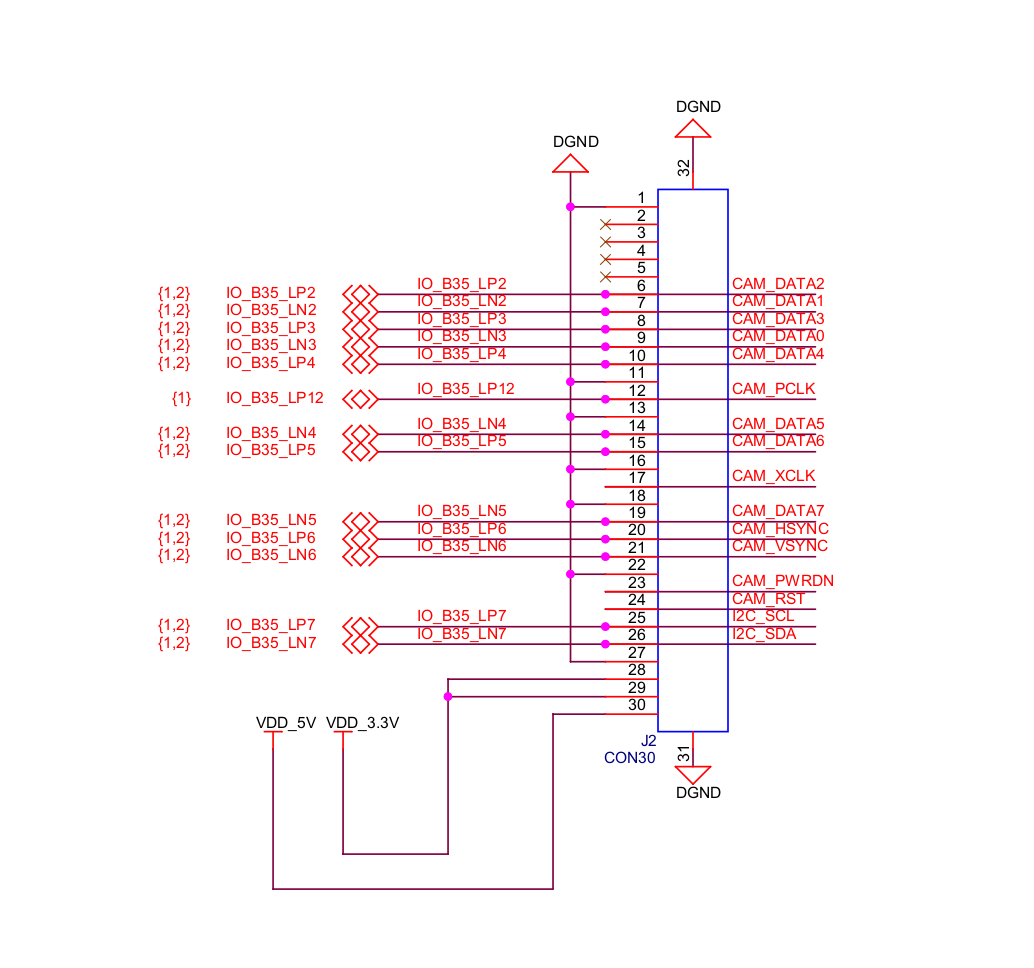
\includegraphics[width=\textwidth]{img/cam-schematic.png}
  \caption{Schemat portu DVP na płytce rozszerzeniowej IO-Cape}
  \label{cam-schematic}
\end{figure}

Dołączenie samego sygnału zegara do konektora FPC byłoby problematyczne, więc zdecydowano się na zastosowanie 
adaptera\footnote{https://kamami.pl/zlacza-ffc-fpc-zif/579387-adapter-zlacza-fpcffc-05mm-30-pin-na-dip.html} złącza FPC/FFC o 
rastrze 0,5 mm na otwory DIP raster 2,54 mm. Dzięki temu możliwe było podłączenie modułu kamery przy użyciu przewodów do 
złącza J3 płytki rozszerzeniowej IO-Cape \cite{ZturnIOCapeSchematic}.


\begin{figure}[!h]
  \centering
  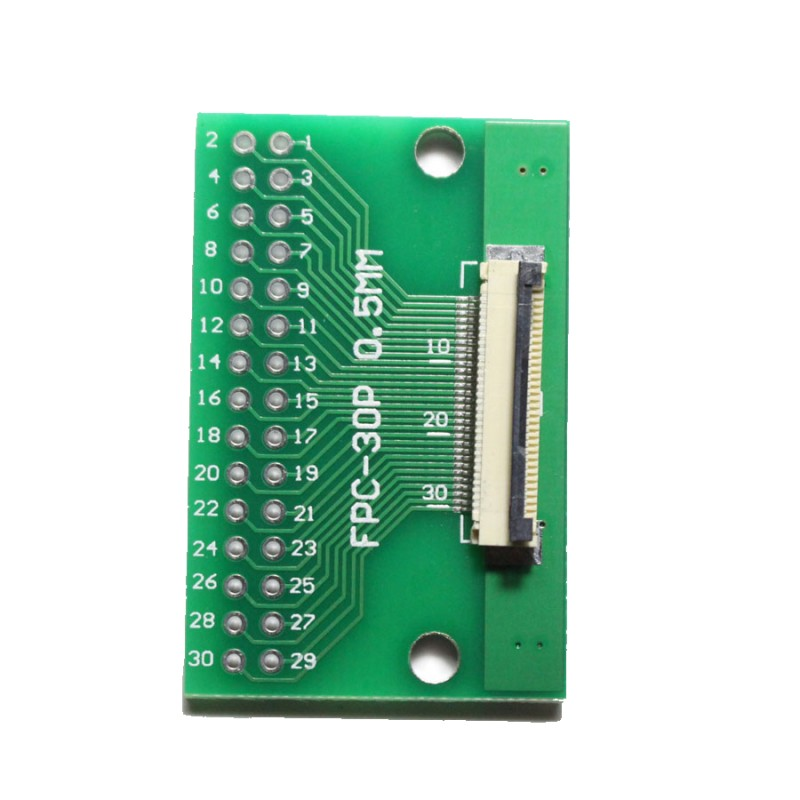
\includegraphics[width=0.8\textwidth]{img/dvp-adapter.jpg}
  \caption{Adapter złącza FPC/FFC o rastrze 0,5 mm na otwory DIP}
  \label{cam-schematic}
\end{figure}


Po podłączeniu kamery, zainstalowaniu odpowiednich sterowników i \emph{device-tree} oraz przeskanowaniu magistrali $I^2C$ 
przy użyciu narzędzia \emph{i2c-tools}, moduł kamery zwraca poprawnie swój adres. Jednak sterownik sensora kamery \emph
{ov2659.c} nie rozpoznaje podłączonego urządzenia. 

\subsubsection{Moduł MY-CAM002B}

Z uwagi na ograniczony czas projektu zdecydowano się na użycie modułu kamery MY-CAM002U USB Digital Camera Module (Rys.\ref
{cam-usb}). Moduł umożliwia rejestrowanie obrazu w 30 klatkach na sekundę przy rozdzielczości 1280x640 pikseli i jest tańszy 
od modułu MY-CAM011B. Główną zaletą tego modułu jest łatwość podłączenia sprzętu zarówno do płytki Z-turn Board, jak i do 
komputera PC, co w znacznym stopniu przyspieszyło debugowanie. 

\begin{figure}[!h]
  \centering
  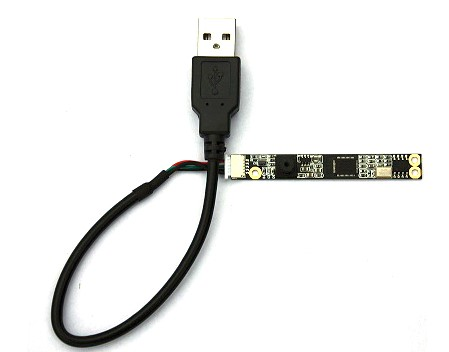
\includegraphics[width=0.8\textwidth]{img/MY-CAM001U.jpg}
  \caption{Moduł kamery MY-CAM002U USB Digital Camera Module}
  \label{cam-usb}
\end{figure}

Kamera po podłączeniu do komputera PC działała poprawnie, bez wprowadzania jakichkolwiek zmian w systemie, zarówno w 
dystrybucji Ubuntu, jak i w systemie Windows. Po dodaniu odpowiednich sterowników do jądra i uruchomieniu systemu Petalinux 
na płytce Z-turn Board, w systemie pojawiły się pliki urządzenia pod nazwą \emph{/dev/video0} oraz \emph{/dev/video1}, co 
umożliwiło odebranie obrazu przy pomocy interfejsu V4L2 (ang. \emph{Video for Linux 2}) oraz OpenCV.
